% Technical appendix master file (camera-ready, NeurIPS 2026 E&D).
% Placed after the references and before the checklist, as the official 2026 template
% orders them; appendices do not count toward the 10 content pages.
% One file per section; each file begins with its own \section{...}. After \appendix the
% sections are lettered A, B, C, ... in the order of the \input lines below.
%
% \PENDING marks a number that the final numbers pass fills from the grid runs
% (SPINEPS: /rs/rs_grp_oschome/go2432/data/ctsp_april/.../neurips_spineps/score_v212/REPORT.md;
%  v11: /rs/rs_grp_oschome/go2432/neurips_v11/out/{ts,ens}/SUMMARY.md). It prints a red
% "[pending]". THE PDF MUST NOT BE UPLOADED WHILE ANY \PENDING REMAINS: fill every slot, or
% cut the section (and the main-text sentences that point to it; see INTEGRATE.md).
\providecommand{\PENDING}{\textcolor{red}{\textbf{[pending]}}}
%
% Written 2026-09-27 with the camera-ready corrections:
\section{Release used, records and the evaluated split}
\label{app:release}

\paragraph{The April 2026 release and Zenodo v11.}
The segmentation experiments ran on the April 2026 release
(\S\ref{sec:dataset}). Its separate spine-only and
pelvic-only records, for patients whose two source
annotations lie on different acquisitions, are what the
partial-annotation protocol (\S\ref{sec:partial}) trains
on. The current archived version, v11, differs from it as
follows: one record per patient (802 records), each
separate-mode patient's missing pelvis completed on the
spine's series by out-of-fold pseudolabelling; VerSe-native
identifiers (L1--L6 = 20--25, sacrum 26, hips 30/31) with
femora, per-level ribs, lumbar ribs and surgical hardware
added as further classes; hip-laterality corrections on 22
records and hand corrections on five; both Castellvi reads
and their consensus in the manifest; and the CT images
supplied by TCIA series crosswalk and rebuild script, with
a HuggingFace mirror carrying the volumes. The 802 patients
and the 33 Castellvi-graded patients are the same in both.

\paragraph{Records and split.}
\label{app:split}
Table~\ref{tab:scan_stats} gives the composition and the
record sets the experiments used. The train, validation
and test manifests are those of the release's 1 May 2026
revision, redrawn two days before training began; the
converter sends the train and validation manifests to the
cross-validation pool and holds out the test manifest.
The five folds are the release's patient-level fold
assignment copied onto the pool's records, so within the
pool no patient spans two validation folds. Each
validation-manifest record therefore trains four of the
five fold models, and each fold's best checkpoint is
selected on that fold's validation records, never on the
test manifest.

\begin{table}[h]
\caption{\dataset{} composition (April 2026 release) and
the record sets of the experiments.}
\label{tab:scan_stats}
\centering
\small
\begin{tabular}{lrr}
\toprule
\bfseries Set & \bfseries Patients & \bfseries Records \\
\midrule
Fused (spine + pelvis)                         & 342 & 342 \\
Separate-mode (spine record + pelvic record)   & 351 & 702 \\
Spine-only / pelvic-only                       & 89 / 20 & 89 / 20 \\
All                                            & 802 & 1{,}153 \\
\quad with spine / pelvic labels               & --- & 782 / 713 \\
\quad of the 33 LSTV patients                  & 33 & 53 \\
\midrule
Train manifest                                 & 639 & 805 \\
Validation manifest                            & 170 & 174 \\
Cross-validation pool (train + validation)     & --- & 979 \\
Test manifest (held out)                       & 167 & 174 \\
\bottomrule
\end{tabular}
\end{table}

The test manifest is a record-level split stratified by
LSTV class and match type. Of its 174 records (167
patients), 82 records from 75 patients are
patient-disjoint from the pool: 52 fused and 16
single-mode patients (14 spine-only, 2 pelvic-only), and
7 separate-mode patients with both records held out. The
other 92 are separate-mode records (52 pelvic, 40 spine)
whose sibling---the patient's other acquisition, labelled
only for the other region---is in the pool (81 from the
train manifest, 11 from the validation manifest) and
trains four of the five fold models. Among the 33 LSTV
patients, 167, 672 and 125 are held out entirely; 401,
555, 123 and 4 have an LSTV-tagged held-out record and a
pool record (tagged normal for 401, 555 and 123 by the
refinement rule of \S\ref{sec:partial}, ambiguous for 4);
104 has its spine record (tagged sacr\_count) in the pool
and its pelvic record, tagged normal, held out. The pool
siblings of 104 and 4 carry an LSTV tag and were
therefore oversampled in the folds that trained on them.
By record, the 33 LSTV patients' 53 records are 44 in the
pool (28 LSTV-tagged) and 9 held out (7 LSTV-tagged).
Table~\ref{tab:castellvi_dist} counts patients: the Pool
and Test columns overlap in one patient (4) by tag, and in
five (401, 555, 123, 4, 104) by any record.

\paragraph{The Normal stratum.}
The Normal rows of Tables~\ref{tab:comparison}
and~\ref{tab:baseline} hold 167 records from 161
patients: 165 records of 159 normal patients and the
pelvic records of LSTV patients 104 (count-style
sacralization) and 672 (lumbarization), tagged normal
because they carry no spine labels. Removing those two
records moves the Normal ensemble sacrum mean from 0.9719
to 0.9717, the merged hip from 0.9884 to 0.9882 and the
mean foreground Dice from 0.9658 to 0.9655; spine classes
and junction-DSC are unaffected.

\paragraph{What is public.}
Neither the April release's 1{,}153 records nor the
evaluated split is at a location this paper cites. The
Zenodo archive (v11) and the OpenSpineConsortium
HuggingFace mirror hold the 802-record v11 layout, and the
archive's \texttt{splits\_5fold.json} is the patient-level
fold assignment over the 802 patients, with no test split.
Its per-patient subtype map is not the six-way taxonomy of
this paper: like the unmerged control's
(Appendix~\ref{app:unmerged}), it has no count-style class
and tags one more patient lumbarization (lumbarization 15,
sacralization 15, semi-sacralization 2, ambiguous 2, normal
768), so strata drawn from it differ from those of
Tables~\ref{tab:sota_stratified}
and~\ref{tab:castellvi_dist}. The six-way subtypes are the
\texttt{lstv\_phenotype} field of the v11 manifest
(lumbarization 14, count-style sacralization 9, full
sacralization 6, semi-sacralization 2, ambiguous 2, empty
for the 769 normal patients).
The anonymous HuggingFace dataset available during review
had been re-uploaded on 18--20 May 2026 with a different
record-level split, which shares 25 of the 174 held-out
records. Until the April manifests and the held-out record
list are published, the segmentation results cannot be
reproduced exactly from public files.
      % A  Release used, records and the evaluated split
\section{Castellvi grades before and after review}
\label{app:castellvi}

The reviewed version's Table~4 was a single grade column
dated 6 May 2026, described there as a joint annotation by
the two residents with no independent inter-rater
scoring. An intermediate sheet of 23 August 2026 added
second reads of five cases (175, 189, 215, 261, 267) and
changed one grade (175, IIIb$\to$Ib). The two full reads,
complete by 4 September 2026, and their consensus are
what this paper reports (Table~\ref{tab:castellvi_hist}).
Reader~2's grades for those five cases equal the 23 August
second reads, including 189 and 215, where reader~1
differs, so at least part of reader~2's grading predates
September.

\begin{table}[h]
\caption{Castellvi distribution over the 33 LSTV patients
in each grade sheet.}
\label{tab:castellvi_hist}
\centering
\small
\begin{tabular}{lrrrrrr}
\toprule
\bfseries Sheet & \bfseries Ib & \bfseries IIa & \bfseries IIb & \bfseries IIIa & \bfseries IIIb & \bfseries IV \\
\midrule
May 2026 (reviewed Table~4)       & 1 & 2 & 4 & 3 & 19 & 4 \\
August 2026 (five second reads)   & 2 & 2 & 4 & 3 & 18 & 4 \\
Reader 1 (by 4 September 2026)    & 2 & 4 & 6 & 1 & 16 & 4 \\
Reader 2 (by 4 September 2026)    & 1 & 2 & 6 & 3 & 17 & 4 \\
Consensus (4 September 2026)      & 2 & 4 & 6 & 1 & 16 & 4 \\
\bottomrule
\end{tabular}
\end{table}

\paragraph{What changed.}
Five grades differ between the May sheet and the
consensus: tokens 22 and 140 (IIIa$\to$IIa), 123 and 125
(IIIb$\to$IIb), and 175 (IIIb$\to$Ib). In the four
III$\to$II changes the May sheet and reader~2 agreed on
Type~III and the consensus took reader~1's Type~II; 175 is
Ib in both reads. Type~I therefore rose from 1
to 2 (175 and 215, both lumbarizations), IIIb fell from
19 (58\%) to 16 (48\%), and full sacralization went from
all Type~III/IV to IIa~1, IIb~2, IIIb~1, IV~2. All nine
count-style sacralizations are IIIb in the May sheet and
in both reads.

\paragraph{Agreement.}
The six disagreements (reader~1/reader~2) are 22 IIa/IIIa,
123 IIb/IIIb, 125 IIb/IIIb, 140 IIa/IIIa, 189 IIIb/IIb and
215 Ib/IIb. The consensus equals reader~1 on all 33 cases
and reader~2 on 27. The May sheet agrees with reader~2 on
30 of 33 and with reader~1 on 28; the files do not record
who filled it. A case bootstrap of the full-grade $\kappa$
(patients resampled, $B{=}10{,}000$) gives 0.53--0.91,
against the Fleiss--Cohen--Everitt interval 0.55--0.92 of
\S\ref{sec:castellvi}. The per-reader files carry no
timestamps, so whether the two reads were made
independently of each other cannot be checked from them.
The September sheet also records a count of
non-rib-bearing vertebrae in a single column: the sheet's
count of 6 (as in May) carries reader~1's annotation of 4
or 5 in 7 of 33 cases (the six full sacralizations and
semi-sacralization 22); the count is not used in this
paper.
  % B  Castellvi grades before and after review
\section{The unmerged control: split, loss and readings}
\label{app:unmerged}

\paragraph{Split and subtype map.}
The unmerged control (\S\ref{sec:unmerged}) was trained on
26--31 July 2026 on a later conversion of the same 1{,}153
records: another record-level 805/174/174 split with a
979-record cross-validation pool, fold train/validation
sizes 765/214, 791/188, 798/181, 774/205 and 788/191. It
shares 25 of the 174 records held out in this paper; 149
of those 174 lie in its pool, among them held-out LSTV
records of patients 167 (its validation fold~3), 672
(fold~0), 123 (fold~2), 4 (fold~1) and 104 (fold~4). Its
subtype map has no count-style class (count-style
sacralization is merged into sacralization) and tags 15
records lumbarization, one more than this paper's
taxonomy (token 500).

\paragraph{Loss and sampling.}
Cross-entropy weights were
$[0.5,1,1,1,1,1.5,4.0,2.0,1,1]$ (background, L1--L4, L5,
L6, sacrum, hips), the merged model's weights plus L6 at
4.0. Patch-level L6 biasing was configured at probability
0.60 and forced an L6 patch in 0.98--1.41\% of
foreground-forced draws per fold; the merged model ran
without patch-level biasing.

\begin{table}[h]
\caption{Unmerged control per fold: validation
lumbarization records (tokens), share of GT-L6 voxels
predicted L5 (mean and range over the final 100 epochs;
final epoch), and validation pseudo-Dice over the same
epochs.}
\label{tab:unmerged_folds}
\centering
\small
\begin{tabular}{llcccc}
\toprule
\bfseries Fold & \bfseries Lumbarization (val) & \bfseries L6$\to$L5, mean (range) & \bfseries Final & \bfseries L6 Dice & \bfseries L5 Dice \\
\midrule
0 & 500, 672, 737 & 83.0\% (29.0--99.9) & 99.9\% & 0.092 & 0.950 \\
1 & none          & ---                 & ---    & 0.099 & 0.928 \\
2 & 189, 261, 666 & 65.4\% (26.0--99.5) & 93.3\% & 0.047 & 0.936 \\
3 & 167, 267, 344 & 66.3\% (17.9--98.2) & 64.7\% & 0.134 & 0.951 \\
4 & 175, 215, 587 & 96.8\% (64.3--100)  & 99.8\% & 0.014 & 0.907 \\
\bottomrule
\end{tabular}
\end{table}

Fold~4's validation lumbarizations include both Type~I
patients (175 and 215). Fold~1's confusion block reports no
lumbarization case in any of its 500 epochs.

\paragraph{The figure quoted during review.}
A range of 84.7--99.4\% was quoted on 27 July 2026, about
17:00. At that time only folds 0 and 4 were running, at
epochs 279 and 277 of 500; folds 1--3 started on 28 July.
The logs admit one moment at which the latest single-epoch
readings of folds 0 and 4 were 84.7\% and 99.4\%: 27 July,
14:02--14:06 (epochs 257 and 255). The figures in
\S\ref{sec:unmerged} are from the completed runs, under
the rule stated there.
   % C  The unmerged control: split, loss and readings
\section{Training and hardware details}
\label{app:training}

\paragraph{Network.}
nnU-Net v2 ResEnc-M planner, \texttt{3d\_fullres},
\texttt{nnUNetResEncUNetPlans\_100G}: a 7-stage residual
encoder with $n_\text{features}{=}[32,64,128,256,320,320,320]$
and $n_\text{blocks}{=}[1,3,4,6,6,6,6]$, $3^3$ kernels,
$2^3$ strides, instance normalization and deep supervision
at 5 levels; a 9-channel output (background and eight
foreground classes), with the ignore label (9) masked from
the loss. In the class-reweighted DC\_and\_CE loss,
$\mathbf{w}{=}[0.5,1,1,1,1,1.5,2.0,1,1]$, the 1.5 on
last\_lumbar targets the lumbosacral boundary and the 2.0
on sacrum the junction the Castellvi grade describes.

\paragraph{Hardware.}
Training ran on H200 NVL (140\,GB HBM3e) with 24 CPU
workers. The preprocessed data were unpacked once per
job to a 1.7\,TB local-NVMe cache, replacing network-file
reads that throttled at 21\,MB/s when five folds read at
once.
   % D  Network and hardware details moved from Section 7
\section{Per-class \texorpdfstring{$n$}{n} and intervals for the stratified results}
\label{app:ci}

Table~\ref{tab:ci} gives, for each row of
Table~\ref{tab:sota_stratified}, the number of patients
scorable for each class and a 95\% case-bootstrap interval
for the mean: patients resampled with replacement within
the subgroup, $B{=}10{,}000$, percentile, seed 20260926.
Where three or fewer patients are scorable the
per-patient values are listed instead. A class is
unscored for a patient when none of its records carries
that region's labels. The Normal$-$Any-LSTV junction drop of 29.0 points
has a two-sample case-bootstrap interval of 9.9--47.4
points; under the stricter rule of \S\ref{sec:audit} (5
LSTV patients) the drop is 35.5 points (15.1--55.5). Hips
are omitted: no row differs from Normal by more than 0.01.

\begin{table}[h]
\caption{\sota{} zero-shot: 95\% case-bootstrap interval
of each Table~\ref{tab:sota_stratified} mean, with the
number of scorable patients ($n$) below it; per-patient
values where three or fewer are scorable.}
\label{tab:ci}
\centering
\footnotesize
\setlength{\tabcolsep}{4pt}
\begin{tabular}{lccccccc}
\toprule
\bfseries Subgroup & \bfseries L1 & \bfseries L2 & \bfseries L3 & \bfseries L4 & \bfseries L5 & \bfseries Sac & \bfseries Jxn DSC \\
\midrule
Normal              & .909--.931 & .906--.929 & .920--.937 & .928--.944 & .931--.945 & .816--.817 & .820--.828 \\
\quad $n$           & 750 & 750 & 750 & 750 & 750 & 683 & 334 \\[2pt]
Any LSTV            & .535--.820 & .459--.763 & .385--.660 & .226--.513 & .175--.458 & .810--.833 & .348--.722 \\
\quad $n$           & 31 & 31 & 31 & 31 & 31 & 29 & 7 \\[2pt]
Lumbarization       & .740--.953 & .710--.943 & .545--.817 & .184--.602 & .099--.507 & .816--.854 & .221, .234, .618 \\
\quad $n$           & 14 & 14 & 14 & 14 & 14 & 11 & 3 \\[2pt]
Sacr.\ (count)      & .011--.532 & .000--.296 & .000--.163 & .000--.001 & .000--.000 & .805--.822 & .467, .927 \\
\quad $n$           & 9 & 9 & 9 & 9 & 9 & 8 & 2 \\[2pt]
Semi-sacralization  & .951 & .951 & .951 & .955 & .956 & .821, .828 & none \\
\quad $n$           & 1 & 1 & 1 & 1 & 1 & 2 & 0 \\[2pt]
Sacr.\ (full)       & .339--.952 & .297--.953 & .317--.953 & .371--.954 & .500--.953 & .801--.851 & .433, .838 \\
\quad $n$           & 5 & 5 & 5 & 5 & 5 & 6 & 2 \\[2pt]
Ambiguous           & .951, .952 & .949, .953 & .863, .901 & .649, .707 & .336, .413 & .730, .813 & none \\
\quad $n$           & 2 & 2 & 2 & 2 & 2 & 2 & 0 \\
\bottomrule
\end{tabular}
\end{table}

\paragraph{Our model, per case.}
No population interval is possible for our held-out LSTV
strata, which hold one to three records per class.
Table~\ref{tab:baseline} gives the mean of the five fold
checkpoints; the per-record values below are the five-fold
ensemble's, which is what the per-case evaluation file
holds. On the three held-out lumbarization records
(167, 401\_r1, 672), L1 is .805, 1.000 and .797; L2 .492,
1.000 and .403; L3 .175, .988 and .006; L4 .0003, .675 and
.0003; and last\_lumbar .645, .725 and .666 (ensemble means
.867, .632, .389, .225 and .678, against the checkpoint
means .872, .611, .377, .213 and .698 of
Table~\ref{tab:baseline}). Two of the three (167 and 672)
shift through the upper lumbars; 401\_r1 does not.
          % E  Per-class n and case-bootstrap intervals (added 2026-09-27, second pass)
% Added 2026-09-27, third pass (drafts promised to reviewer Fbco; slots for the final numbers pass):
% Appendix F: Background (promised to reviewer Fbco: "a Background section (LSTV subtypes;
% Castellvi I to IV; the VERIDAH architecture)"). Integrated 2026-09-27 (third pass) from the
% verified draft scratchpad/neurips_promises/drafts/app_background.tex; notes in
% app_background_NOTES.md. Uses sec:dataset, sec:castellvi, tab:castellvi_dist, sec:audit,
% sec:unmerged, app:spineps and app:tsv3 (appendix/spineps.tex). If the SPINEPS section is cut,
% replace "(Appendix~\ref{app:spineps})" with "(the current release)"; if the total_v3 slot is
% cut, end the footnote with "It was not evaluated here."
%
% Every factual sentence is sourced. Where each number was checked (27 Sep 2026):
%  Konin & Walz 2010, AJNR 31:1778: 4-30%; Castellvi definitions; morphology ("varying degrees
%    of lumbarization, such as ..." - the S1 features are examples, not all required); p.1778
%    (first page, not 1779; checked page-by-page in MANUAL_REFS/KONIN_WALZ.pdf) "does not provide
%    information relevant to accurate enumeration of the involved segment".
%  Castellvi 1984: classification; 60 of 200 myelography patients (PubMed 6495013 abstract,
%    saved in paper/mpda/_schehr/sources.json). Full text NOT read; the type definitions are
%    Konin & Walz's restatement and are attributed to them.
%  Carrino 2011: 147 subjects; LSTV associated with anomalous total count, OR 7.4 (Europe PMC
%    abstract). Sekharappa 2014: 3 x 1,000; 8.1/14/16.9%; type I "not called a transitional
%    vertebra in our study" (PMC3939369). Hanhivaara 2022: 310 of 1,468 (21.1%), Castellvi
%    classification used, type I findings reported (Europe PMC abstract). Nagata 2025: 551
%    whole-spine CTs, 16.3%; sacralization = 23 presacral, lumbarization = 25 (PubMed abstract).
%    Lian 2018: counting caudally from C2 is the gold standard (abstract).
%  Liebl 2021 (VerSe'20, PMC8553749): Wigh's definition (ribs < 38 mm on both sides = TLTV) is
%    quoted, but VerSe'20 itself labels a vertebra thoracic if at least one rib > 38 mm (with
%    diagonal downward alignment) and LUMBAR if both are shorter; Castellvi II-IV graded ("only
%    Castellvi II-IV were classified"); "did not segment vertebrae that showed partial fusion
%    with the sacrum (Castellvi grades III and IV)"; variants per subject in Suppl. Table 1.
%  VerSe ids: github.com/anjany/verse README ("20-25: lumbar spine: L1-L6", "28: ... T13").
%  CTSpine1K (Deng et al.): "Every vertebra (from C1 to L6) is labeled with integer values from
%    1 to 25"; "containing L6 (resulting from sacral lumbarization) or losing L5 (resulting from
%    lumbar sacralization)"; "the DSC of L6 is almost 0 ... the existence of L6 confuses the
%    model, resulting in prediction dislocations".
%  VERIDAH (arXiv:2601.14066v1, the only version): Sec. 2.1-2.2, Tables 2, 3, 5, Figs 1D, 5.
%    The label head is stated as "23 classes" while the cost set C is "all 24 vertebra labels"
%    C1..L5 (the paper's own inconsistency), so the text says only "no T13 or L6 class". The CT
%    cohort is "in-house" (not called private). Locations come from instance segmentations; the
%    method "requires the centroids of vertebrae beforehand".
%  SPINEPS paper (Eur Radiol 35:1178): MRI only; "the instance labels are counted from top to
%    bottom regardless of the field of view or the presence of enumeration abnormalities".
%  SPINEPS 2.1.2 (PyPI, uploaded 24 Sep 2026): CT_semantic, CT_instance, ct_labeling
%    (DenseNet169); post-map "L1..L6 -> 20..25, T13 -> 28" (scout_spineps/s212/.../phase_labeling.py).
%  TotalSegmentator: 'total' map = C1..L5, sacrum, S1, no L6/T13 (map_to_binary.py in the
%    2.4.0 wheel, 117 classes; README "Class details" table); vertebrae_S1 new in v2
%    (improvements_in_v2.md); the audit ran TotalSegmentator==2.4.0
%    (docker/Dockerfile.totalsegmentator @ c53d2dc). Footnote, re-checked 27 Sep 2026: the
%    PyPI wheels 2.15.0 (1 Jul 2026), 2.17.0 and 2.18.0 (12 Aug) all define
%    class_map["total_v3"] = total with [26]="vertebrae_L6" (2.12.0-2.14.0 do not);
%    map_tasks_config.py maps total_v3 to task ids 831-837 with version "v3.0.0-weights"; the
%    GitHub release v3.0.0-weights (pre-release, published 2026-09-07, body "Add weights for
%    v3.0.0") carries Dataset831-837 zips, and a range request for 836 returned HTTP 206, so the
%    weights ARE downloadable (not license-gated: total_v3 is not in commercial_models). Only the
%    "download all" script download_pretrained_weights.py omits 831-837. CHANGELOG and README
%    do not mention total_v3 or L6.
%  MDPA (arXiv:2609.22760v1, describes release v11): "no scan in this dataset contains C2";
%    v11 adds lower thoracic levels, ribs, lumbar ribs and classes for L6 and T13. April has 1,153
%    records, not v11's 802: the 351 extra series are the other acquisition of the same CT
%    colonography exams (ACRIN 6664), so "no C2" carries over by field of view, not by identity
%    of series. (v11 Table S3 lists id 1 "C1" in 2 records and id 6 "C6" in 1 record, isolated
%    labels with no C2-C5 or T1-T2 anywhere; the highest contiguous level is T3. Not checked
%    further; it does not bear on this appendix.)

\section{Background: transitional vertebrae, Castellvi grading and \VERIDAH{}}
\label{app:background}

\paragraph{Enumeration and transition.}
The spine usually has seven cervical, twelve thoracic and five lumbar vertebrae. An
enumeration anomaly gives eleven or thirteen thoracic or four or six lumbar vertebrae; a
transitional vertebra is a border segment with features of both neighbouring
regions~\citep{Moller2026VERIDAH:Sequences,Konin2010LumbosacralRelevance}. The two co-occur: a
lumbosacral transitional vertebra (LSTV) is associated with an anomalous total
count~\citep{Carrino2011EffectImaging}. An LSTV is either
sacralization of the lowest lumbar segment, from a broadened transverse process to complete
fusion with the sacrum, or lumbarization of the uppermost sacral segment, which may
articulate rather than fuse and may show lumbar-type facets or a fully sized S1--S2
disc~\citep{Konin2010LumbosacralRelevance}. The same words also name counts:
\citet{Nagata2025LSTVWholeSpine} define sacralization as 23 presacral vertebrae and
lumbarization as 25. Rib conventions differ as well: \VERIDAH{} calls any vertebra with a true
rib thoracic, whatever the rib's length~\citep{Moller2026VERIDAH:Sequences}; VerSe'20 calls it
thoracic only if one rib exceeds 38\,mm, and lumbar if both are
shorter~\citep{Liebl2021VerSeData}. The reference standard for numbering
remains a count from C2 on whole-spine imaging~\citep{Lian2018LSTVNumeration}. Reported LSTV
prevalence is 4--30\%~\citep{Konin2010LumbosacralRelevance},
21.1\% of 1{,}468 lumbar MRIs~\citep{Hanhivaara2022LSTV} and 16.3\% of 551 whole-spine CTs by
count~\citep{Nagata2025LSTVWholeSpine}. It varies with the population, from 8.1\% to 16.9\%
across three clinic groups in one series, which did not count Castellvi type~I as
transitional~\citep{Sekharappa2014LumbosacralSignificance}.

\paragraph{The six subtypes in these terms.}
The taxonomy of \S\ref{sec:dataset} inherits its sources' conventions. CTSpine1K numbers
C1--L6 as 1--25 and attributes an L6 to sacral lumbarization and a missing L5 to lumbar
sacralization~\citep{Deng2021CTSpine1K:Tomography}; \texttt{lumb} and
\texttt{sacr\_count} are these counts. A count does not place the anomaly: six lumbar
vertebrae can follow eleven thoracic ones, and four can follow a
T13 (\citealp{Moller2026VERIDAH:Sequences}, Figs.~1D and~5), and no scan here, all CT
colonography of the abdomen and pelvis, contains C2~\citep{Schwing2026CTSpinoPelvic1KArxiv}.
\texttt{sacralization} and \texttt{semisacralization} rest on CTPelvic1K's undocumented
filename tag. The April release has no thoracic, T13 or rib class, so the thoracolumbar border
cannot be checked on it; the current release (v11) adds thoracic levels, ribs, lumbar ribs and
a T13 class~\citep{Schwing2026CTSpinoPelvic1KArxiv}.

\paragraph{Castellvi classification.}
\citet{Castellvi1984LumbosacralDefects} typed the transitional segment mainly by the
morphology of its transverse process. As restated by \citet{Konin2010LumbosacralRelevance}, with \emph{a} marking a
unilateral and \emph{b} a bilateral finding, type~I (Ia, Ib) is a dysplastic transverse
process at least 19\,mm in craniocaudal width. Type~II (IIa, IIb) is an enlarged transverse process forming a
diarthrodial joint with the sacrum. Type~III (IIIa, IIIb) is complete osseous fusion of the
transverse process to the sacrum. Type~IV is type~II on one side and type~III on the other.
The grade ``does not provide information relevant to accurate enumeration of the involved
segment''~\citep[p.~1778]{Konin2010LumbosacralRelevance}, which is why \S\ref{sec:castellvi}
treats it as orthogonal to the count; type~IIIb occurs here at lumbar counts of four, five
and six (Table~\ref{tab:castellvi_dist}). VerSe'20 classified only types II--IV, lists each
subject's variants, and left vertebrae partly fused to the sacrum (III, IV)
unsegmented~\citep{Liebl2021VerSeData}; \VERIDAH{}'s reference labels
call any Castellvi-bearing vertebra a sacralized lumbar one, and it outputs no
grade~\citep{Moller2026VERIDAH:Sequences}.

\paragraph{\VERIDAH{} and SPINEPS.}
\VERIDAH{}~\citep{Moller2026VERIDAH:Sequences} labels vertebrae whose positions are given
(the paper takes them from instance segmentations). A 3-D DenseNet169 classifies a crop
centred on each vertebra with four heads: vertebra label (no T13 or L6 class), region,
transition (last cervical, first thoracic, last thoracic, first lumbar, last lumbar, or none)
and visibility. For training, T13 and L6 are relabelled T12 and L5, so an extra vertebra is a repeated T12 or L5 that only the transition
head separates, and anomalous cases are drawn four times per epoch. A sequence predictor
combines the heads into a path cost weighted by each vertebra's visibility and minimises it by
dynamic programming under hard constraints: consecutive, spatially ordered labels; 11--13
thoracic and 4--6 lumbar; at most one repeated T12 and one repeated L5, renamed T13 and L6.
On 365 in-house test CTs enriched for anomalies it labelled every vertebra correctly in
99.18\% of subjects, against 77.81\% for the method of \citet{Meng2022VertebraeMLMI}, and
recalled 97.22\% of lumbar enumeration anomalies; in its ablation one label head without the
predictor recalls 30.56\%, with it 63.89\%, and four heads without it 30.56\%.
SPINEPS~\citep{Moller2024SPINEPSautomaticSegmentation} is a semantic-then-instance
segmentation of T2-weighted MRI whose instances are counted top to bottom ``regardless of the
field of view or the presence of enumeration abnormalities''; \VERIDAH{} supplies the
labelling step and ships with its code~\citep{Moller2026VERIDAH:Sequences}. SPINEPS~2.1.2
(Appendix~\ref{app:spineps}) runs CT models before the \VERIDAH{} labeller and writes \VerSe{}
ids, L6 as 25 and T13 as 28~\citep{MollerSPINEPSSoftware}; the peer-reviewed SPINEPS paper
covers MRI only.

\paragraph{Why a missing class shifts labels.}
A segmenter gives each voxel one label from a fixed vocabulary. \VerSe{} numbers L1--L6 as
20--25 and T13 as 28~\citep{VerSeRepo}, and CTSpine1K and the April release have an L6 class;
the \texttt{total} task of \TS{} (version 2.4.0 was audited) has C1--L5, the sacrum and S1 but
no L6 or T13~\citep{Wasserthal2023TotalSegmentator:Images,TotalSegmentatorCode}.\footnote{Since
version 2.15.0 (1 July 2026) the \TS{} package has also defined a \texttt{total\_v3} task whose
class map puts \texttt{vertebrae\_L6} where \texttt{total} has \texttt{vertebrae\_S1}; its
weights were posted as a GitHub pre-release on 7 September 2026, and neither the changelog
nor the README describes it~\citep{TotalSegmentatorCode}. It postdates the
benchmark of \S\ref{sec:audit}; Appendix~\ref{app:tsv3} evaluates it under the same protocol.} Given
six lumbar-type segments and five lumbar labels, a model must reuse a label or give a segment
a thoracic, sacral or no label; on lumbarized spines \TS{} gives the L6 the L5 label in two of
three scorable junctions, and its lumbar Dice falls level by level toward the sacrum
(\S\ref{sec:audit}). An L6 output label is necessary but not sufficient, and it need not be a
trained class. CTSpine1K's own nnU-Net baseline scored an L6 Dice of almost
zero~\citep{Deng2021CTSpine1K:Tomography}; our unmerged control, trained with an L6
class, still labels most ground-truth L6 voxels in its validation patches L5
(\S\ref{sec:unmerged}); and \VERIDAH{} as published has no L6 class, yet names an L6 as a
repeated L5 that its transition head and sequence predictor
place~\citep{Moller2026VERIDAH:Sequences}.
           % F  Background: transitional vertebrae, Castellvi, VERIDAH
% Appendix section: dataset-construction figure (promised to reviewer Fbco in the rebuttal:
% "We add a Background section ... and a dataset-construction figure").
% Appendix G. Integrated 2026-09-27 (third pass) from the verified draft
% scratchpad/neurips_promises/drafts/app_construction.tex; the figure is
% figs/fig_app_construction.pdf (TikZ source: drafts/fig_app_construction.tex). Bib entry
% Schwing2026CTSpinoPelvic1KArxiv is in bib/references.bib. Refers to app:release
% (appendix/release_split.tex) and sec:dataset (main text).
% Every number and its source: app_construction_NOTES.md.
\section{How the April 2026 release was built}
\label{app:construction}

Figure~\ref{fig:construction} traces the April 2026 release
(\S\ref{sec:dataset}) from its three sources to the records
the experiments used. It is adapted from the construction
figure of the dataset
article~\citep{Schwing2026CTSpinoPelvic1KArxiv}, which describes
the later v11 release; the steps only v11 has are left out
and are listed in Appendix~\ref{app:release}. The placement
step counts 804 patients, 352 of them separate and 90
spine-only. The orientation review excluded one separate
patient, and one placed spine-only patient is absent from
the export for a reason the export did not record, so the
release holds 351 separate and 89 spine-only patients.
A front-to-back mirror is not a rotation. In the two of the
nine checked, tokens 75 and 480, the released CT shows the
liver on the left. The six hip-label swaps match the labels
to the side of the image, which for 480 is the mirror of the
patient's; the other seven were not rendered.

\begin{figure}[ht]
\centering
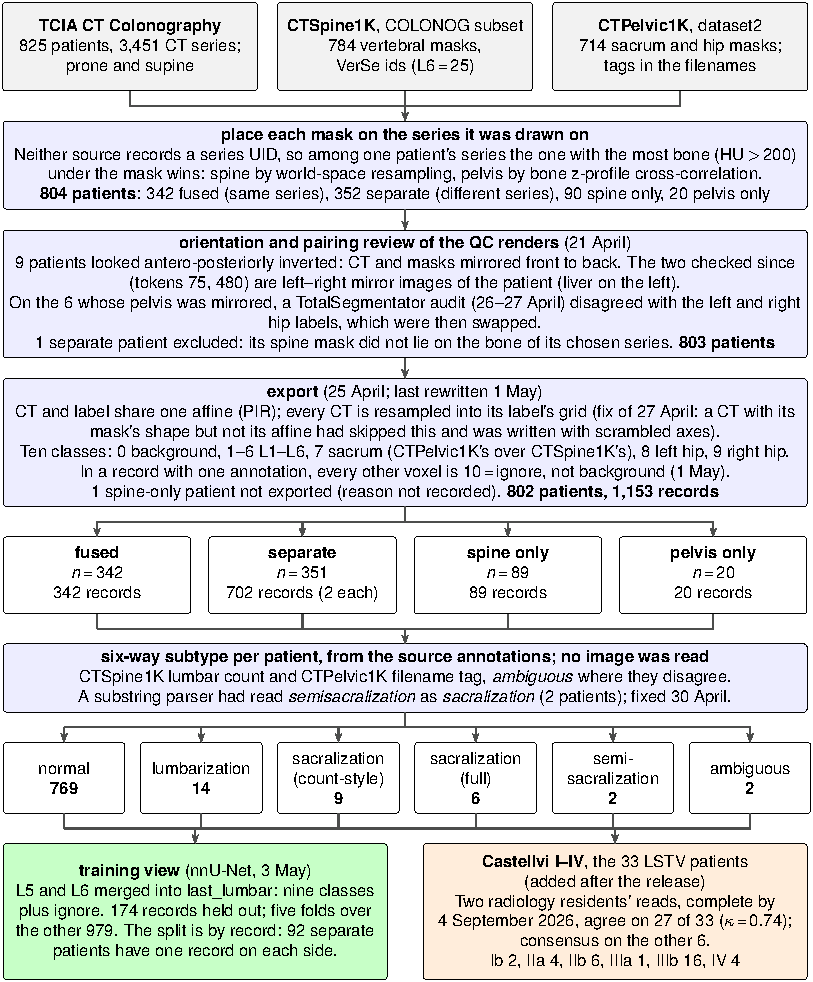
\includegraphics[width=\linewidth]{figs/fig_app_construction.pdf}
\caption{Construction of the April 2026 release of \dataset{},
on which every segmentation experiment here was run: 802
patients, 1{,}153 records; \textit{n} counts patients. Grey,
sources; blue, the April pipeline; green, the training view;
orange, added after the release. Adapted from Fig.~1 of the dataset
article~\citep{Schwing2026CTSpinoPelvic1KArxiv}, which describes a
later release (v11).}
\label{fig:construction}
\end{figure}
  % G  How the April 2026 release was built (figure)
% Appendix H: comparison with other CT collections (promised to reviewer Fbco in the author
% response of 27 Jul 2026). Integrated 2026-09-27 (third pass) from the verified draft
% scratchpad/neurips_promises/drafts/app_comparison.tex; the licence line now also gives ours
% per host, and note g points to the total_v3 slot.
%
% Needs only what neurips_2026.tex already loads (booktabs; amssymb for \checkmark) and its
% macros \dataset, \TS, \VerSe, \VERIDAH. Its bib entries are merged into bib/references.bib.
% Every cell and its source: drafts/app_comparison_NOTES.md.
% The CTSpinoPelvic1K row is the April 2026 release (1,153 records, 802 patients).
% Label tab:dataset_comparison (tab:comparison is taken by the baselines table).
\section{Comparison with other CT collections}
\label{app:comparison}

Table~\ref{tab:dataset_comparison} compares \dataset{} with the CT collections that label
anatomy at the lumbosacral junction; each cell was checked against the collection's own
paper or data page. \VerSe{} comes closest in intent: it labels L6 and T13, lists anatomical
variants per subject and grades Castellvi II--IV, but it segments neither the sacrum nor a
transitional vertebra partially fused to it, so its type~III and IV cases cannot be scored
at L5/S1. CTSpine1K labels L6 but no pelvis, and its nnU-Net baseline already scored L6 at
a Dice of 0 on all three of its test sets, with shifted predictions on lumbarization and
sacralization cases (its Table~2 and Fig.~4)~\citep{Deng2021CTSpine1K:Tomography}, which is
consistent with the unmerged control of \S\ref{sec:unmerged}. Among these collections, only
\dataset{} puts numbered lumbar levels including L6, the sacrum and both hip bones on the
same patients, with a per-patient LSTV label and, for its 33 LSTV patients, a Castellvi grade.

\begin{table}[h]
\caption{CT collections labelling the lumbosacral junction. \checkmark{}
present; (\checkmark) partial; -- absent; letters refer to the notes. Patients in
parentheses where reported and different from scans. Pelvis: S sacrum, H hip bones,
F femora. Unified: spine and pelvis in the same patients. Adapted from Table~I of the
dataset article~\citep{Schwing2026CTSpinoPelvic1KArxiv}, which describes a later release.}
\label{tab:dataset_comparison}
\centering
\small
\setlength{\tabcolsep}{3pt}
\begin{tabular}{@{}lrlcccccc@{}}
\toprule
\bfseries Collection & \bfseries Scans & \bfseries Levels & \bfseries Pelvis
  & \bfseries Unified & \bfseries LSTV & \bfseries Six-way & \bfseries Castellvi
  & \bfseries Public \\
 & (patients) & labelled & & cohort & labels & subtype & grade & data \\
\midrule
\VerSe{}
  & 374 (355) & C1--L6, T13\textsuperscript{a} & --
  & -- & (\checkmark)\textsuperscript{b} & -- & (\checkmark)\textsuperscript{c} & \checkmark \\
CTSpine1K
  & 1{,}005 & C1--L6\textsuperscript{d} & --
  & -- & (\checkmark)\textsuperscript{d} & -- & -- & \checkmark \\
CTPelvic1K
  & 1{,}184 & lumbar, 1 class\textsuperscript{e} & S, H
  & (\checkmark)\textsuperscript{e} & (\checkmark)\textsuperscript{f} & -- & -- & \checkmark \\
\TS{}
  & 1{,}204 & C1--L5\textsuperscript{g} & S, H, F
  & (\checkmark)\textsuperscript{g} & -- & -- & -- & \checkmark \\
\VERIDAH{} CT cohort
  & 1{,}536 & C1--L6, T13\textsuperscript{h} & --\textsuperscript{h}
  & -- & (\checkmark)\textsuperscript{h} & -- & --\textsuperscript{h} & -- \\
\dataset{}
  & 1{,}153 (802)\textsuperscript{i} & L1--L6 & S, H
  & \checkmark\textsuperscript{i} & \checkmark\textsuperscript{j} & \checkmark\textsuperscript{j}
  & \checkmark\textsuperscript{k} & \checkmark\textsuperscript{i} \\
\bottomrule
\end{tabular}

\smallskip
\footnotesize
\raggedright
\textsuperscript{a}Identifiers 1--25 (C1--L6) and 28 (T13); sacrum and coccyx not
labelled~\citep{VerSeRepo}; 374 scans of 355 patients~\citep{Sekuboyina2021VerSe:Images}.
\textsuperscript{b}VerSe'20 was assembled partly from reports of anatomical variants and
lists them per subject; 85 of its cases have six lumbar vertebrae~\citep{Liebl2021VerSeData}.
\textsuperscript{c}Castellvi II--IV graded in VerSe'20 (IIa 35, IIb 25, IIIa 14, IIIb 28,
IV 7), types 0 and I pooled; the sacrum and vertebrae partially fused to it (III, IV) are
not segmented~\citep{Liebl2021VerSeData}.
\textsuperscript{d}Identifiers 1--25 (C1--L6); 784 of the 1{,}005 volumes are COLONOG.
Its Table~1 counts 17 lumbarization and 11 sacralization cases, ungraded; the authors list
their IDs with the data~\citep{Deng2021CTSpine1K:Tomography}.
\textsuperscript{e}Four classes: lumbar spine (one class), sacrum, left and right hip, on
the same scan, cropped to the pelvic region; patient count not
reported~\citep{Liu2021DeepModels}.
\textsuperscript{f}Undocumented tags in ten of the 713 COLONOG mask filenames on Zenodo:
sacralization 7, semisacralization 2, hard\_sacralization 1~\citep{Liu2020CTPelvic1KData,Schwing2026CTSpinoPelvic1KArxiv}.
\textsuperscript{g}The cited paper's dataset (v1, 104 classes)~\citep{Wasserthal2023TotalSegmentator:Images,Wasserthal2022TSDatasetV1};
v2.0.1 has 1{,}228 scans and 117 classes and adds
S1~\citep{Wasserthal2023TSDatasetV2,TotalSegmentatorCode}; neither has L6 (the software's
later \texttt{total\_v3} task has an L6 class; Appendix~\ref{app:tsv3}). Every
structure in the field of view is labelled; how many scans hold both lumbar spine and
pelvis is not reported.
\textsuperscript{h}In-house cohort, patient count not reported; reference labels include
T13 and L6, merged into T12 and L5 for training; enumeration anomalies are labelled by
count, and a Castellvi transitional vertebra is labelled sacralized lumbar whatever its type;
lumbar and sacral vertebrae are distinguished, but no sacral or pelvic segmentation is
described; code and weights public, no image release
described~\citep{Moller2026VERIDAH:Sequences}.
\textsuperscript{i}Records of the April 2026 release used here (Appendix~\ref{app:release}).
Spine and pelvis for 693 of 802 patients: on one series for 342, on two acquisitions of the
same patient (two records) for 351; 89 spine-only, 20 pelvis-only. Public as v11 (the same
802 patients, one record each); the April records and evaluated split are not yet at a
cited location.
\textsuperscript{j}For all 802 patients (33 LSTV), from the source masks' lumbar counts and
filename tags, not image reads (\S\ref{sec:dataset}); the six subtypes are listed per
patient in the v11 manifest (\texttt{lstv\_phenotype}).
\textsuperscript{k}Types I--IV for all 33 LSTV patients: a two-resident consensus completed
in September 2026, after the April release, and distributed from Zenodo v8 onward
(\S\ref{sec:castellvi}, Appendix~\ref{app:castellvi}); normal patients not screened for
type I.
Licences: \VerSe{} CC BY-SA 4.0; CTSpine1K CC BY-NC-SA 4.0; CTPelvic1K CC BY-NC-SA (paper)
or CC BY 4.0 (Zenodo record); \TS{} data CC BY 4.0; \dataset{} CC BY-NC-SA 4.0 on Zenodo, the
archive of record, and CC BY-NC 4.0 on the dataset card of its HuggingFace mirror (checked
27 September 2026).
\end{table}

\paragraph{How the benchmark will be used.}
Its first use is as a stratified test: a CT segmenter or vertebra labeller is scored per
LSTV subtype with junction-DSC and voxel confusion at L5/S1,
each stratum reported with its $n$ (\S\ref{sec:protocol}), which is what a model claiming
readiness for surgical planning should show. Adding an L6 class did not remove the L5/L6
collision at this sample size (\S\ref{sec:unmerged}), and the signal that separates a last
lumbar vertebra from its neighbour is a count that one patch does not reliably contain, so
the benchmark is meant as the test set for counting-aware and two-stage ``segment, then
number'' designs, such as a segmenter feeding \VERIDAH{}'s sequence predictor
(\S\ref{sec:discussion}). Its LSTV strata are small (33 patients, 7 with an LSTV-tagged
held-out record; Wilson intervals for strata of 3--4 cases start at 44--51\%,
\S\ref{sec:limits-test-set}), so it exposes a failure mode and its direction rather than
ranking methods that differ by a few points.
   % H  Comparison with other CT collections
% Appendix I: SPINEPS under the benchmark protocol (promised to reviewer Fbco: "We will
% additionally report SPINEPS evaluated under the same protocol in the revised paper"), with the
% slot for TotalSegmentator's later total_v3 task. Skeleton written 2026-09-27 (third pass).
%
% FILL FROM (final numbers pass):
%   SPINEPS  /rs/rs_grp_oschome/go2432/data/ctsp_april/.../neurips_spineps/score_v212/REPORT.md
%            grid jobs 40481323 (GPU array, 1,153 records) -> 40481314 (score) -> 40481315 (aggregate);
%            status: bash /rs/rs_grp_oschome/go2432/data/ctsp_april/run/status_spineps.sh
%            Fill only if REPORT.md shows 0 GT-gate mismatches (no "DO NOT REPORT" banner).
%   total_v3 NOT RUN, no job submitted (Greg decides whether it enters the paper; SCOUT_spineps,
%            RESUME "Findings" 1). If it is not run: delete the total_v3 column of
%            tab:spineps_l6 and the \paragraph{...total_v3} below, and change the three main-text
%            pointers to app:tsv3 (Section 3, Limitations) and the footnote in background.tex and
%            note g in dataset_comparison.tex to "not evaluated here".
% Method facts below are from scratchpad/neurips_promises/SCOUT_spineps.md sections 0-5.
% The TS column of tab:spineps_l6: L5 < 0.5 rows recomputed 2026-09-27 from
% Desktop/NeurIPS/bm/benchmark_per_case.csv by neurips_integrate/l5_subgroups.py (it reproduces the
% published 10/14, 9/9, 9/750); GT-L6 rows and junction rows are the published Section 3 values
% (189: 0.8% from the v11 scout). Junction DSC here is the Table 1 scorer's window
% (benchmark_totalseg.py @ c53d2dc, junction_analysis); if the final pass redefines Table 1's
% junction window (v11 defect B), redefine this row the same way.
\section{SPINEPS under the benchmark protocol}
\label{app:spineps}

\paragraph{What was run.}
SPINEPS~2.1.2~\citep{MollerSPINEPSSoftware}, released on 24 September 2026, segments a CT
with a semantic and an instance model and names the instances with the \VERIDAH{}
labeller, writing \VerSe{} identifiers with L6 as 25 and T13 as 28
(Appendix~\ref{app:background}); unlike 2.1.1, it labels CT without rotating each
vertebra's crop, so the two versions can name the same spine differently. It ran on the
native CT of each of the 1{,}153 April records with the three CT models it ships, without
bias-field correction and otherwise at its defaults; a record on which it fails counts as
a failure, as \TS{}'s one failure did. Its identifiers were mapped onto the April scheme
(20--24 to L1--L5, 25 to L6, 26 to sacrum; thoracic levels, T13 and discs to background)
and scored with the unchanged functions of the \TS{} benchmark script: per-class DSC gated
by record type, the patient-level merge, the six-way subgroups and the junction window of
Table~\ref{tab:sota_stratified}. Before scoring, each record's ground-truth quantities
(classes present and, on fused records, the junction window and its voxel counts) were
checked against the 30 April \TS{} run; a mismatch would void the tables. SPINEPS has no
hip class, so hips are not applicable (N/A). Its sacrum includes the S1 body, which the
published \TS{} sacrum scores as a miss; the like-for-like \TS{} sacrum is the S1-inclusive
row of Table~\ref{tab:v11}. \PENDING{} records failed.

\begin{table}[h]
\caption{SPINEPS~2.1.2 zero-shot on \dataset{} (April release), stratified as
Table~\ref{tab:sota_stratified}: per-class DSC, $n$ patients. Sacrum includes the S1 body.
Hips: N/A (no hip class). Junction DSC over the window of
Table~\ref{tab:sota_stratified} on fused records ($n_\text{jxn}$).}
\label{tab:spineps_strat}
\centering
\small
\resizebox{\linewidth}{!}{%
\begin{tabular}{lrccccccccr}
\toprule
\bfseries Subgroup & \bfseries $n$ &
\bfseries L1 & \bfseries L2 & \bfseries L3 & \bfseries L4 & \bfseries L5 & \bfseries L6 &
\bfseries Sac & \bfseries Jxn DSC & \bfseries $n_\text{jxn}$ \\
\midrule
All cases                         & \PENDING & \PENDING & \PENDING & \PENDING & \PENDING & \PENDING & \PENDING & \PENDING & \PENDING & \PENDING \\
Normal                            & \PENDING & \PENDING & \PENDING & \PENDING & \PENDING & \PENDING & \PENDING & \PENDING & \PENDING & \PENDING \\
\midrule
Any LSTV                          & \PENDING & \PENDING & \PENDING & \PENDING & \PENDING & \PENDING & \PENDING & \PENDING & \PENDING & \PENDING \\
\quad Lumbarization               & \PENDING & \PENDING & \PENDING & \PENDING & \PENDING & \PENDING & \PENDING & \PENDING & \PENDING & \PENDING \\
\quad Sacralization (count-style) & \PENDING & \PENDING & \PENDING & \PENDING & \PENDING & \PENDING & \PENDING & \PENDING & \PENDING & \PENDING \\
\quad Semi-sacralization          & \PENDING & \PENDING & \PENDING & \PENDING & \PENDING & \PENDING & \PENDING & \PENDING & \PENDING & \PENDING \\
\quad Sacralization (full)        & \PENDING & \PENDING & \PENDING & \PENDING & \PENDING & \PENDING & \PENDING & \PENDING & \PENDING & \PENDING \\
\quad Ambiguous                   & \PENDING & \PENDING & \PENDING & \PENDING & \PENDING & \PENDING & \PENDING & \PENDING & \PENDING & \PENDING \\
\bottomrule
\end{tabular}%
}
\end{table}

\begin{table}[h]
\caption{Level naming at the lumbosacral junction under one protocol: the audited \TS{}~2.4.0
(\texttt{total} task, \S\ref{sec:audit}), SPINEPS~2.1.2 and \TS{} \texttt{total\_v3}. Per
patient unless stated; brackets, Wilson 95\% intervals. GT-L6 voxel shares are over the
junction window of the three junction-scorable lumbarization patients (tokens).}
\label{tab:spineps_l6}
\centering
\small
\setlength{\tabcolsep}{4pt}
\resizebox{\linewidth}{!}{%
\begin{tabular}{@{}llll@{}}
\toprule
\bfseries Quantity & \bfseries \TS{} 2.4.0 \texttt{total} & \bfseries SPINEPS 2.1.2 & \bfseries \TS{} \texttt{total\_v3} \\
\midrule
\multicolumn{4}{@{}l}{\itshape L5 DSC $<$ 0.5, patients with a scorable L5} \\
\quad Lumbarization               & 10/14 (45--88\%)     & \PENDING & \PENDING \\
\quad Sacralization (count-style) & 9/9 (70--100\%)      & \PENDING & \PENDING \\
\quad Sacralization (full)        & 1/5 (4--62\%)        & \PENDING & \PENDING \\
\quad Semi-sacralization          & 0/1 (0--79\%)        & \PENDING & \PENDING \\
\quad Ambiguous                   & 2/2 (34--100\%)      & \PENDING & \PENDING \\
\quad Any LSTV                    & 22/31 (53--84\%)     & \PENDING & \PENDING \\
\quad Normal                      & 9/750 (0.6--2.3\%)   & \PENDING & \PENDING \\
\midrule
\multicolumn{4}{@{}l}{\itshape L6 emitted (any L6 voxel)} \\
\quad Records                     & 0/1{,}152 (no class) & \PENDING{}/\PENDING & \PENDING \\
\quad Lumbarization patients      & 0/14                 & \PENDING{}/14 & \PENDING \\
\quad Normal patients             & 0/768                & \PENDING{}/768 & \PENDING \\
\midrule
\multicolumn{4}{@{}l}{\itshape GT-L6 voxels in the junction window named \ldots{} (167, 699, 189)} \\
\quad L5                          & 95.2, 97.1, 0.8\%    & \PENDING & \PENDING \\
\quad L6                          & 0, 0, 0\%            & \PENDING & \PENDING \\
\midrule
\multicolumn{4}{@{}l}{\itshape Junction DSC, fused records} \\
\quad Normal                      & 0.824 ($n{=}334$)    & \PENDING & \PENDING \\
\quad Any LSTV                    & 0.534 ($n{=}7$)      & \PENDING & \PENDING \\
\quad Lumbarization               & 0.357 ($n{=}3$)      & \PENDING & \PENDING \\
\bottomrule
\end{tabular}%
}
\end{table}

\paragraph{What the tables show.}
\PENDING{}

\paragraph{\TS{} \texttt{total\_v3}.}
\label{app:tsv3}
\TS{}~2.15.0 (1 July 2026) added a \texttt{total\_v3} task whose class map puts
\texttt{vertebrae\_L6} where the audited \texttt{total} task has \texttt{vertebrae\_S1}; its
weights were posted as a GitHub pre-release on 7 September
2026~\citep{TotalSegmentatorCode}. Both came after the benchmark of \S\ref{sec:audit} ran
(30 April 2026), whose findings therefore describe the \texttt{total} task of 2.4.0, not
\TS{} as shipped today. Its column of Table~\ref{tab:spineps_l6} applies the same
protocol, with \texttt{vertebrae\_L6} mapped to L6. \PENDING{}
              % I  SPINEPS under the benchmark protocol (+ TS total_v3 slot)
% Appendix J: the reproducible layer rerun on Zenodo v11. Integrated 2026-09-27 (third pass) from
% scratchpad/neurips_v11/drafts/app_v11.tex. Changes on integration: "on \PENDING{} of 112 cases"
% became "on \PENDING{} of \PENDING{} cases" (the same paragraph gives 115 admissible patients and
% nothing records why 112; the final pass states the count SUMMARY.md reports), and the
% \providecommand{\PENDING} moved to appendix/appendix.tex. Main-text edit (1) below is made
% (Section 5 "Release used" now points here); decision (2) is still Greg's.
% Grid status 2026-09-27 ~02:00: 40480728 (TS, 16), 40480730 (ensemble, 8), 40480731-33 all PENDING.
% Numbers marked \PENDING{} come from the grid run in /rs/rs_grp_oschome/go2432/neurips_v11 (JOBS.txt):
%   TS rows       out/ts/SUMMARY.md      (L6 emission; the junction-window GT-L6 list; the L5<0.5 table, V11-M/AM
%                                          column; Table-1 V11-M/AM and V11-M/S1 blocks; the positive-control line)
%   Ensemble rows out/ens/SUMMARY.md     (LSTV per-case table, v11_manual column; the reproduction line)
% Fill a cell only if that SUMMARY.md carries no NOT REPORTABLE banner.
% Two edits to the main text go with this section (not made here; src is read-only for this workflow):
%   (1) Section 5 "Release used" ends "Nothing here was recomputed on v11."; that becomes false.
%       Replace with e.g. "Appendix~\ref{app:v11} reruns the zero-shot benchmark and the released ensemble on v11."
%   (2) DECISION for Greg, row marked (S1) below: the published TS sacrum (0.817) counts TS's separate S1-body
%       class as a miss (scout SCOUT.md section 0 A; fixed in benchmark_totalseg.py on 15 June, never rerun).
%       Keeping this row puts the corrected value next to the abstract's "0.817 -> 0.969" / "+15.3 pts", so it
%       stands only together with a decision about those main-text numbers. Delete the row to defer.

\section{Results on the current release (v11)}
\label{app:v11}

\paragraph{What differs, and what does not.}
The archived v11
(\href{https://doi.org/10.5281/zenodo.22797014}{10.5281/zenodo.22797014})
keeps the April release's 802 patients and 33
Castellvi-graded patients but not its records
(Appendix~\ref{app:release}): it holds one volume per
patient, so the 351 separate-mode pelvic CTs are absent,
and the pelvis of 440 spine-series volumes and the spine
of 20 pelvis-only volumes are pseudolabels, which
Table~\ref{tab:v11} does not score. The images are
unchanged: 799 of the 802 v11 CTs are byte-identical
(SHA-256) to the April file for the same patient and
series, and the other three could not be compared because
the April copy stored each under a filename shared with
another patient. So are the manual labels, to within a
few voxels: over the 779 records labelled in both
releases, every lumbar level of more than 1{,}000 voxels
agrees at Dice $\geq 0.996$ (below 0.999 twice: an L1
that lost 0.7\% of its voxels to v11's new lumbar-rib
class and an L2 trimmed by 0.2\%), the 31 LSTV patients
with a spine label agree at $\geq 0.9989$ at every level,
the 362 sacra at $\geq 0.994$ and the 362 hip pairs voxel
for voxel, and no level is renumbered.

\paragraph{What was rerun.}
\sota{}~2.4.0 ran on all 802 v11 CTs in the April
container with the April call, adding the S1 body to the
requested structures; scored as in April (S1 dropped,
April labels), it reproduces the 30 April per-record Dice
to within $10^{-3}$ on \PENDING{} of \PENDING{} records.
The five released fold checkpoints ran on the 115
held-out patients whose v11 CT was their April test
image: 75 with no acquisition in the cross-validation
pool and 40 whose other acquisition was in it ($^\ast$).
The 52 held-out patients whose v11 CT was a pool image,
LSTV patients 104, 123 and 4 among them, are excluded. On
the April labels the ensemble reproduces the 6 May
per-case Dice to within $10^{-3}$ on \PENDING{} of \PENDING{}
cases.

\begin{table}[h]
\caption{\sota{} (zero-shot, per patient) and the released
five-fold ensemble (held-out patients) on the April 2026
release as published and rerun on v11, scoring only
manually labelled structures. Junction-window rows are
fused records. $^\ast$: the patient's other acquisition
was in the training pool. Brackets: Wilson 95\% intervals.}
\label{tab:v11}
\centering
\small
\begin{tabular}{@{}lll@{}}
\toprule
\bfseries Quantity & \bfseries April (published) & \bfseries v11 \\
\midrule
\multicolumn{3}{@{}l}{\itshape \sota{}, zero-shot} \\
\textsc{L6} labels emitted                              & 0 / 1{,}152 records          & \PENDING{} / 802 volumes \\
GT-L6 voxels labelled L5, junction window: 167, 699     & 95.2\%, 97.1\%               & \PENDING{}, \PENDING{} \\
\quad 189 (the rest background)                         & 0.8\%                        & \PENDING{} \\
L5 DSC $<$ 0.5: lumbarization                           & 10/14 (45--88\%)             & \PENDING{} \\
\quad count-style sacralization                         & 9/9 (70--100\%)              & \PENDING{} \\
\quad normal                                            & 9/750 (0.6--2.3\%)           & \PENDING{} \\
L1--L5 DSC, all patients (range of level means)         & 0.906--0.914 ($n{=}801$)     & \PENDING{} \\
L4 / L5 DSC, lumbarization                              & 0.388 / 0.291 ($n{=}14$)     & \PENDING{} \\
L5 DSC, any LSTV                                        & 0.314                        & \PENDING{} \\
Sacrum DSC, S1 body scored as a miss                    & 0.817 ($n{=}712$)            & \PENDING{} ($n{=}362$) \\
Sacrum DSC, S1 body counted as sacrum (S1)              & ---                          & \PENDING{} ($n{=}362$) \\
\midrule
\multicolumn{3}{@{}l}{\itshape Released ensemble, held-out} \\
last\_lumbar DSC, lumbarization 167, 672, 401$^\ast$    & 0.645, 0.666, 0.725          & \PENDING{} \\
last\_lumbar DSC, full sacralization 125                & 0.623                        & \PENDING{} \\
L4 DSC, count-style sacralization 555$^\ast$            & 0.032                        & \PENDING{} \\
Junction DSC, 167                                       & 0.950                        & \PENDING{} \\
\bottomrule
\end{tabular}
\end{table}
          % J  Results on the current release (v11)
